\documentclass[11pt,a4paper,]{article}
\usepackage{lmodern}

\usepackage{amssymb,amsmath}
\usepackage{ifxetex,ifluatex}
\usepackage{fixltx2e} % provides \textsubscript
\ifnum 0\ifxetex 1\fi\ifluatex 1\fi=0 % if pdftex
  \usepackage[T1]{fontenc}
  \usepackage[utf8]{inputenc}
\else % if luatex or xelatex
  \usepackage{unicode-math}
  \defaultfontfeatures{Ligatures=TeX,Scale=MatchLowercase}
\fi
% use upquote if available, for straight quotes in verbatim environments
\IfFileExists{upquote.sty}{\usepackage{upquote}}{}
% use microtype if available
\IfFileExists{microtype.sty}{%
\usepackage[]{microtype}
\UseMicrotypeSet[protrusion]{basicmath} % disable protrusion for tt fonts
}{}
\PassOptionsToPackage{hyphens}{url} % url is loaded by hyperref
\usepackage[unicode=true]{hyperref}
\hypersetup{
            pdftitle={Gender birth rate trend analysis in the United States},
            pdfborder={0 0 0},
            breaklinks=true}
\urlstyle{same}  % don't use monospace font for urls
\usepackage{geometry}
\geometry{a4paper, centering, text={16cm,25cm}}
\usepackage[style=authoryear-comp,]{biblatex}
\addbibresource{references.bib}
\usepackage{color}
\usepackage{fancyvrb}
\newcommand{\VerbBar}{|}
\newcommand{\VERB}{\Verb[commandchars=\\\{\}]}
\DefineVerbatimEnvironment{Highlighting}{Verbatim}{commandchars=\\\{\}}
% Add ',fontsize=\small' for more characters per line
\usepackage{framed}
\definecolor{shadecolor}{RGB}{248,248,248}
\newenvironment{Shaded}{\begin{snugshade}}{\end{snugshade}}
\newcommand{\AlertTok}[1]{\textcolor[rgb]{0.94,0.16,0.16}{#1}}
\newcommand{\AnnotationTok}[1]{\textcolor[rgb]{0.56,0.35,0.01}{\textbf{\textit{#1}}}}
\newcommand{\AttributeTok}[1]{\textcolor[rgb]{0.13,0.29,0.53}{#1}}
\newcommand{\BaseNTok}[1]{\textcolor[rgb]{0.00,0.00,0.81}{#1}}
\newcommand{\BuiltInTok}[1]{#1}
\newcommand{\CharTok}[1]{\textcolor[rgb]{0.31,0.60,0.02}{#1}}
\newcommand{\CommentTok}[1]{\textcolor[rgb]{0.56,0.35,0.01}{\textit{#1}}}
\newcommand{\CommentVarTok}[1]{\textcolor[rgb]{0.56,0.35,0.01}{\textbf{\textit{#1}}}}
\newcommand{\ConstantTok}[1]{\textcolor[rgb]{0.56,0.35,0.01}{#1}}
\newcommand{\ControlFlowTok}[1]{\textcolor[rgb]{0.13,0.29,0.53}{\textbf{#1}}}
\newcommand{\DataTypeTok}[1]{\textcolor[rgb]{0.13,0.29,0.53}{#1}}
\newcommand{\DecValTok}[1]{\textcolor[rgb]{0.00,0.00,0.81}{#1}}
\newcommand{\DocumentationTok}[1]{\textcolor[rgb]{0.56,0.35,0.01}{\textbf{\textit{#1}}}}
\newcommand{\ErrorTok}[1]{\textcolor[rgb]{0.64,0.00,0.00}{\textbf{#1}}}
\newcommand{\ExtensionTok}[1]{#1}
\newcommand{\FloatTok}[1]{\textcolor[rgb]{0.00,0.00,0.81}{#1}}
\newcommand{\FunctionTok}[1]{\textcolor[rgb]{0.13,0.29,0.53}{\textbf{#1}}}
\newcommand{\ImportTok}[1]{#1}
\newcommand{\InformationTok}[1]{\textcolor[rgb]{0.56,0.35,0.01}{\textbf{\textit{#1}}}}
\newcommand{\KeywordTok}[1]{\textcolor[rgb]{0.13,0.29,0.53}{\textbf{#1}}}
\newcommand{\NormalTok}[1]{#1}
\newcommand{\OperatorTok}[1]{\textcolor[rgb]{0.81,0.36,0.00}{\textbf{#1}}}
\newcommand{\OtherTok}[1]{\textcolor[rgb]{0.56,0.35,0.01}{#1}}
\newcommand{\PreprocessorTok}[1]{\textcolor[rgb]{0.56,0.35,0.01}{\textit{#1}}}
\newcommand{\RegionMarkerTok}[1]{#1}
\newcommand{\SpecialCharTok}[1]{\textcolor[rgb]{0.81,0.36,0.00}{\textbf{#1}}}
\newcommand{\SpecialStringTok}[1]{\textcolor[rgb]{0.31,0.60,0.02}{#1}}
\newcommand{\StringTok}[1]{\textcolor[rgb]{0.31,0.60,0.02}{#1}}
\newcommand{\VariableTok}[1]{\textcolor[rgb]{0.00,0.00,0.00}{#1}}
\newcommand{\VerbatimStringTok}[1]{\textcolor[rgb]{0.31,0.60,0.02}{#1}}
\newcommand{\WarningTok}[1]{\textcolor[rgb]{0.56,0.35,0.01}{\textbf{\textit{#1}}}}
\usepackage{longtable,booktabs}
% Fix footnotes in tables (requires footnote package)
\IfFileExists{footnote.sty}{\usepackage{footnote}\makesavenoteenv{long table}}{}
\IfFileExists{parskip.sty}{%
\usepackage{parskip}
}{% else
\setlength{\parindent}{0pt}
\setlength{\parskip}{6pt plus 2pt minus 1pt}
}
\setlength{\emergencystretch}{3em}  % prevent overfull lines
\providecommand{\tightlist}{%
  \setlength{\itemsep}{0pt}\setlength{\parskip}{0pt}}
\setcounter{secnumdepth}{5}

% set default figure placement to htbp
\makeatletter
\def\fps@figure{htbp}
\makeatother


\title{Gender birth rate trend analysis \newline in the United States\huge}

%% MONASH STUFF

%% CAPTIONS
\RequirePackage{caption}
\DeclareCaptionStyle{italic}[justification=centering]
 {labelfont={bf},textfont={it},labelsep=colon}
\captionsetup[figure]{style=italic,format=hang,singlelinecheck=true}
\captionsetup[table]{style=italic,format=hang,singlelinecheck=true}


%% FONT
\RequirePackage{bera}
\RequirePackage[charter,expert,sfscaled]{mathdesign}
\RequirePackage{fontawesome}

%% HEADERS AND FOOTERS
\RequirePackage{fancyhdr}
\pagestyle{fancy}
\rfoot{\Large\sffamily\raisebox{-0.1cm}{\textbf{\thepage}}}
\makeatletter
\lhead{\textsf{\expandafter{\@title}}}
\makeatother
\rhead{}
\cfoot{}
\setlength{\headheight}{15pt}
\renewcommand{\headrulewidth}{0.4pt}
\renewcommand{\footrulewidth}{0.4pt}
\fancypagestyle{plain}{%
\fancyhf{} % clear all header and footer fields
\fancyfoot[C]{\sffamily\thepage} % except the center
\renewcommand{\headrulewidth}{0pt}
\renewcommand{\footrulewidth}{0pt}}

%% MATHS
\RequirePackage{bm,amsmath}
\allowdisplaybreaks

%% GRAPHICS
\RequirePackage{graphicx}
\setcounter{topnumber}{2}
\setcounter{bottomnumber}{2}
\setcounter{totalnumber}{4}
\renewcommand{\topfraction}{0.85}
\renewcommand{\bottomfraction}{0.85}
\renewcommand{\textfraction}{0.15}
\renewcommand{\floatpagefraction}{0.8}


%\RequirePackage[section]{placeins}

%% SECTION TITLES


%% SECTION TITLES
\RequirePackage[compact,sf,bf]{titlesec}
\titleformat*{\section}{\Large\sf\bfseries\color[rgb]{0.7,0,0}}
\titleformat*{\subsection}{\large\sf\bfseries\color[rgb]{0.7,0,0}}
\titleformat*{\subsubsection}{\sf\bfseries\color[rgb]{0.7,0,0}}
\titlespacing{\section}{0pt}{2ex}{.5ex}
\titlespacing{\subsection}{0pt}{1.5ex}{0ex}
\titlespacing{\subsubsection}{0pt}{.5ex}{0ex}


%% TITLE PAGE
\def\Date{\number\day}
\def\Month{\ifcase\month\or
 January\or February\or March\or April\or May\or June\or
 July\or August\or September\or October\or November\or December\fi}
\def\Year{\number\year}

%% LINE AND PAGE BREAKING
\sloppy
\clubpenalty = 10000
\widowpenalty = 10000
\brokenpenalty = 10000
\RequirePackage{microtype}

%% PARAGRAPH BREAKS
\setlength{\parskip}{1.4ex}
\setlength{\parindent}{0em}

%% HYPERLINKS
\RequirePackage{xcolor} % Needed for links
\definecolor{darkblue}{rgb}{0,0,.6}
\RequirePackage{url}

\makeatletter
\@ifpackageloaded{hyperref}{}{\RequirePackage{hyperref}}
\makeatother
\hypersetup{
     citecolor=0 0 0,
     breaklinks=true,
     bookmarksopen=true,
     bookmarksnumbered=true,
     linkcolor=darkblue,
     urlcolor=blue,
     citecolor=darkblue,
     colorlinks=true}

\usepackage[showonlyrefs]{mathtools}
\usepackage[no-weekday]{eukdate}

%% BIBLIOGRAPHY

\makeatletter
\@ifpackageloaded{biblatex}{}{\usepackage[style=authoryear-comp, backend=biber, natbib=true]{biblatex}}
\makeatother
\ExecuteBibliographyOptions{bibencoding=utf8,minnames=1,maxnames=3, maxbibnames=99,dashed=false,terseinits=true,giveninits=true,uniquename=false,uniquelist=false,doi=false, isbn=false,url=true,sortcites=false}

\DeclareFieldFormat{url}{\texttt{\url{#1}}}
\DeclareFieldFormat[article]{pages}{#1}
\DeclareFieldFormat[inproceedings]{pages}{\lowercase{pp.}#1}
\DeclareFieldFormat[incollection]{pages}{\lowercase{pp.}#1}
\DeclareFieldFormat[article]{volume}{\mkbibbold{#1}}
\DeclareFieldFormat[article]{number}{\mkbibparens{#1}}
\DeclareFieldFormat[article]{title}{\MakeCapital{#1}}
\DeclareFieldFormat[article]{url}{}
%\DeclareFieldFormat[book]{url}{}
%\DeclareFieldFormat[inbook]{url}{}
%\DeclareFieldFormat[incollection]{url}{}
%\DeclareFieldFormat[inproceedings]{url}{}
\DeclareFieldFormat[inproceedings]{title}{#1}
\DeclareFieldFormat{shorthandwidth}{#1}
%\DeclareFieldFormat{extrayear}{}
% No dot before number of articles
\usepackage{xpatch}
\xpatchbibmacro{volume+number+eid}{\setunit*{\adddot}}{}{}{}
% Remove In: for an article.
\renewbibmacro{in:}{%
  \ifentrytype{article}{}{%
  \printtext{\bibstring{in}\intitlepunct}}}

\AtEveryBibitem{\clearfield{month}}
\AtEveryCitekey{\clearfield{month}}

\makeatletter
\DeclareDelimFormat[cbx@textcite]{nameyeardelim}{\addspace}
\makeatother

\author{\sf{\Large\textbf{Arindam Baruah}\\\large \href{mailto:abar0090@student.monash.edu}{\nolinkurl{abar0090@student.monash.edu}} (32779267)\\[0.5cm]}}

\date{\sf\Date~\Month~\Year}
\makeatletter
\lfoot{\sf Baruah: \@date}
\makeatother


%%%% PAGE STYLE FOR FRONT PAGE OF REPORTS

\makeatletter
\def\organization#1{\gdef\@organization{#1}}
\def\telephone#1{\gdef\@telephone{#1}}
\def\email#1{\gdef\@email{#1}}
\makeatother
  \organization{ETC 5242 Task 1}

  \def\name{Department of\newline Econometrics \&\newline Business Statistics}

  \telephone{(03) 9905 2478}

  \email{BusEco-Econometrics@monash.edu}

\def\webaddress{\url{http://buseco.monash.edu/ebs/consulting/}}
\def\abn{12 377 614 012}
\def\extraspace{\vspace*{1.6cm}}
\makeatletter
\def\contactdetails{\faicon{phone} & \@telephone \\
                    \faicon{envelope} & \@email}
\makeatother

\usepackage[absolute,overlay]{textpos}
\setlength{\TPHorizModule}{1cm}
\setlength{\TPVertModule}{1cm}

%%%% FRONT PAGE OF REPORTS

\def\reporttype{Report for}

\long\def\front#1#2#3{
\newpage
\begin{textblock}{7}(12.7,28.2)\hfill

\includegraphics[height=0.6cm]{AACSB}~~~

\includegraphics[height=0.6cm]{EQUIS}~~~

\includegraphics[height=0.6cm]{AMBA}
\end{textblock}
\begin{singlespacing}
\thispagestyle{empty}
\vspace*{-1.4cm}
\hspace*{-1.4cm}
\hbox to 16cm{
  \hbox to 6.5cm{\vbox to 14cm{\vbox to 25cm{
    
\includegraphics[width=6cm]{monash2}
    \vfill
    
\includegraphics[width=3.5cm]{MBSportrait}
    \vspace{0.4cm}
    \par
    \parbox{6.3cm}{\raggedright
      \sf\color[rgb]{0.00,0.00,0.70}
      {\large\textbf{\name}}\par
      \vspace{.7cm}
      \tabcolsep=0.12cm\sf\small
      \begin{tabular}{@{}ll@{}}\contactdetails
      \end{tabular}
      \vspace*{0.3cm}\par
      ABN: \abn\par
    }
  }\vss}\hss}
  \hspace*{0.2cm}
  \hbox to 1cm{\vbox to 14cm{\rule{1pt}{26.8cm}\vss}\hss\hfill}
  \hbox to 10cm{\vbox to 14cm{\vbox to 25cm{
      \vspace*{3cm}\sf\raggedright
      \parbox{11cm}{\sf\raggedright\baselineskip=1.2cm
         \fontsize{24.88}{30}\color[rgb]{0.70,0.00,0.00}\sf\textbf{#1}}
      \par
      \vfill
      \large
      \vbox{\parskip=0.8cm #2}\par
      \vspace*{2cm}\par
      \reporttype\\[0.3cm]
      \hbox{#3}%\\[2cm]\
      \vspace*{1cm}
      {\large\sf\textbf{\Date~\Month~\Year}}
   }\vss}
  }}
\end{singlespacing}
\newpage
}

\makeatletter
\def\titlepage{\front{\expandafter{\@title}}{\@author}{\@organization}}
\makeatother

\usepackage{setspace}
\setstretch{1.5}

%% Any special functions or other packages can be loaded here.
\usepackage{booktabs}
\usepackage{longtable}
\usepackage{array}
\usepackage{multirow}
\usepackage{wrapfig}
\usepackage{float}
\usepackage{colortbl}
\usepackage{pdflscape}
\usepackage{tabu}
\usepackage{threeparttable}
\usepackage{threeparttablex}
\usepackage[normalem]{ulem}
\usepackage{makecell}
\usepackage{xcolor}


\begin{document}
\titlepage

{
\setcounter{tocdepth}{2}
\tableofcontents
}
\hypertarget{introduction}{%
\section{Introduction}\label{introduction}}

The current study delineates a detailed analysis of the birth counts for boys and girls born in the country of The United States of America. The study is based on two separate datasets, the first of which contain gender wise birth data from the years of \textbf{1629 to 1710} and the second, containing the gender birth data from the years of \textbf{1940 to 2002} in the country of The United States. Utilisation of statistical techniques and subsequent feature engineering of the current and the historical data would further provide key insights into the changes of gender birth rate in the aforementioned country of interest. While the studies of \textcite{mathews2005trend} and \textcite{owidgenderratio} have uncovered change of birth rates as a result of various socio-economic causes such as demographic changes, \textbf{the current study would however be limited to exploring the key changes in the number of births for girls and boys using statistical methods and feature engineering.}

It is critical to acknowledge that while the study by \textcite{pryzgoda2000definitions} defines the terminologies of ``Sex ratio'' and ``Gender ratio'' as two different statistics, however for the sake of simplicity, these terms may be used interchangeably in the context of the current study.

\hypertarget{label1}{%
\section{Research Questions}\label{label1}}

In this section of the study, the following key research questions pertaining to the new births in The United States will be formulated and further analysed in section \ref{label2} :

\begin{enumerate}
\def\labelenumi{\arabic{enumi}.}
\tightlist
\item
  \textbf{How do the datasets belonging to the periods of 1629-1710 and 1940-2002 differ from one another} ?
\item
  \textbf{How has the birth rate for girls changed over the period of 1940-2002} ?
\item
  \textbf{Are there any similarities in the birth rate of girls between the time periods of 1629-1710 and 1940-2002} ?
\item
  \textbf{Would creating new statistical features allow us to gain better insights into the data} ?
\item
  \textbf{Are boys born in greater proportion to girls during the period of 1940-2002} ?
\end{enumerate}

\hypertarget{label2}{%
\section{Analysis}\label{label2}}

The current section will provide a step by step analysis for each of the formulated research questions of section \ref{label1}.

\hypertarget{query-1}{%
\subsection{Query 1}\label{query-1}}

A basic understanding on the size of the data and the number of entries for the datasets belonging to each of the two time periods will be explored in this section.

\tiny

\begin{Shaded}
\begin{Highlighting}[]
\FunctionTok{head}\NormalTok{(df\_present) }\SpecialCharTok{\%\textgreater{}\%} 
  \FunctionTok{kable}\NormalTok{(}\AttributeTok{caption =} \StringTok{"Preview of the data containing number of boys and girls born in The United States between 1940{-}2002."}\NormalTok{) }\SpecialCharTok{\%\textgreater{}\%} 
  \FunctionTok{kable\_styling}\NormalTok{(}\AttributeTok{bootstrap\_options =} \FunctionTok{c}\NormalTok{(}\StringTok{"bordered"}\NormalTok{,}\StringTok{"hover"}\NormalTok{),}
                                    \AttributeTok{latex\_options =} \StringTok{"HOLD\_position"}\NormalTok{) }
\end{Highlighting}
\end{Shaded}

\begin{table}[H]

\caption{\label{tab:tabpre}Preview of the data containing number of boys and girls born in The United States between 1940-2002.}
\centering
\begin{tabular}[t]{r|r|r}
\hline
year & boys & girls\\
\hline
1940 & 1211684 & 1148715\\
\hline
1941 & 1289734 & 1223693\\
\hline
1942 & 1444365 & 1364631\\
\hline
1943 & 1508959 & 1427901\\
\hline
1944 & 1435301 & 1359499\\
\hline
1945 & 1404587 & 1330869\\
\hline
\end{tabular}
\end{table}
\normalsize

The above code-chunk and its output as observed through table \ref{tab:tabpre} provides us with the glimpse of the dataset. The dataset contains three features. These features are explained as below:

\begin{itemize}
\tightlist
\item
  \textbf{Year} : The year pertaining to the count of new births in the United States.
\item
  \textbf{boys} : The number of births classified as ``boys'' for the corresponding year.
\item
  \textbf{girls} : The number of births classified as ``girls'' for the corresponding year.
\end{itemize}

Let us observe how do the values of the number of births between the periods of 1629-1710 and 1940-2002 vary from one another through tables \ref{tab:sumstatarb} and \ref{tab:sumstatpre} respectively.

\tiny

\begin{Shaded}
\begin{Highlighting}[]
\FunctionTok{summary}\NormalTok{(df\_arb) }\SpecialCharTok{\%\textgreater{}\%} \FunctionTok{kable}\NormalTok{(}\AttributeTok{caption =} \StringTok{"Summary statistics for data between 1629{-}1710."}\NormalTok{) }\SpecialCharTok{\%\textgreater{}\%} 
  \FunctionTok{kable\_styling}\NormalTok{(}\AttributeTok{bootstrap\_options =} \FunctionTok{c}\NormalTok{(}\StringTok{"bordered"}\NormalTok{,}\StringTok{"hover"}\NormalTok{),}
                                    \AttributeTok{latex\_options =} \StringTok{"HOLD\_position"}\NormalTok{) }
\end{Highlighting}
\end{Shaded}

\begin{table}[H]

\caption{\label{tab:sumstatarb}Summary statistics for data between 1629-1710.}
\centering
\begin{tabular}[t]{l|l|l|l}
\hline
  &      year &      boys &     girls\\
\hline
 & Min.   :1629 & Min.   :2890 & Min.   :2722\\
\hline
 & 1st Qu.:1649 & 1st Qu.:4759 & 1st Qu.:4457\\
\hline
 & Median :1670 & Median :6073 & Median :5718\\
\hline
 & Mean   :1670 & Mean   :5907 & Mean   :5535\\
\hline
 & 3rd Qu.:1690 & 3rd Qu.:7576 & 3rd Qu.:7150\\
\hline
 & Max.   :1710 & Max.   :8426 & Max.   :7779\\
\hline
\end{tabular}
\end{table}

\begin{Shaded}
\begin{Highlighting}[]
\FunctionTok{summary}\NormalTok{(df\_present) }\SpecialCharTok{\%\textgreater{}\%} \FunctionTok{kable}\NormalTok{(}\AttributeTok{caption =} \StringTok{"Summary statistics for data between 1940{-}2002."}\NormalTok{) }\SpecialCharTok{\%\textgreater{}\%} 
  \FunctionTok{kable\_styling}\NormalTok{(}\AttributeTok{bootstrap\_options =} \FunctionTok{c}\NormalTok{(}\StringTok{"bordered"}\NormalTok{,}\StringTok{"hover"}\NormalTok{),}
                                    \AttributeTok{latex\_options =} \StringTok{"HOLD\_position"}\NormalTok{) }
\end{Highlighting}
\end{Shaded}

\begin{table}[H]

\caption{\label{tab:sumstatpre}Summary statistics for data between 1940-2002.}
\centering
\begin{tabular}[t]{l|l|l|l}
\hline
  &      year &      boys &     girls\\
\hline
 & Min.   :1940 & Min.   :1211684 & Min.   :1148715\\
\hline
 & 1st Qu.:1956 & 1st Qu.:1799857 & 1st Qu.:1711404\\
\hline
 & Median :1971 & Median :1924868 & Median :1831679\\
\hline
 & Mean   :1971 & Mean   :1885600 & Mean   :1793915\\
\hline
 & 3rd Qu.:1986 & 3rd Qu.:2058524 & 3rd Qu.:1965538\\
\hline
 & Max.   :2002 & Max.   :2186274 & Max.   :2082052\\
\hline
\end{tabular}
\end{table}

\normalsize

As we can clearly observe, the \textbf{magnitude of the boys and girls born during the period of 1940-2002 are much larger than that for the period of 1629-1710} as reported by the study of \textcite{arbuthnot1710ii}. This is expected as a result of the global rise of population owing to factors such as better infrastructure, better lifestyle, better socio-economic factors and improvement in medical sciences.

Let us try to visualise the same through figure \ref{fig:figbirth}.

\tiny

\begin{Shaded}
\begin{Highlighting}[]
\FunctionTok{options}\NormalTok{(}\AttributeTok{scipen =} \DecValTok{999}\NormalTok{) }\CommentTok{\# To remove scientific notation}

\NormalTok{df\_arb\_long }\OtherTok{\textless{}{-}}
  \FunctionTok{pivot\_longer}\NormalTok{(}
\NormalTok{    df\_arb,}
    \AttributeTok{names\_to =} \StringTok{"gender"}\NormalTok{,}
    \AttributeTok{values\_to =} \StringTok{"born"}\NormalTok{,}
    \AttributeTok{cols =} \FunctionTok{c}\NormalTok{(boys, girls)}
\NormalTok{  )}
\NormalTok{pl1 }\OtherTok{\textless{}{-}}
  \FunctionTok{ggplot}\NormalTok{(}\AttributeTok{data =}\NormalTok{ df\_arb\_long, }\FunctionTok{aes}\NormalTok{(}\AttributeTok{x =}\NormalTok{ year, }\AttributeTok{y =}\NormalTok{ born, }\AttributeTok{fill =}\NormalTok{ gender)) }\SpecialCharTok{+} 
  \FunctionTok{geom\_area}\NormalTok{(}\AttributeTok{color =} \StringTok{\textquotesingle{}black\textquotesingle{}}\NormalTok{) }\SpecialCharTok{+} \FunctionTok{theme\_classic}\NormalTok{() }\SpecialCharTok{+} 
  \FunctionTok{ggtitle}\NormalTok{(}\StringTok{"Birth statistics between 1629{-}1710"}\NormalTok{) }\SpecialCharTok{+} 
  \FunctionTok{theme}\NormalTok{(}\AttributeTok{plot.title =} \FunctionTok{element\_text}\NormalTok{(}\AttributeTok{hjust =} \FloatTok{0.5}\NormalTok{),}\AttributeTok{aspect.ratio =} \FloatTok{0.5}\NormalTok{) }\SpecialCharTok{+} 
  \FunctionTok{labs}\NormalTok{(}\AttributeTok{fill =} \StringTok{"Gender"}\NormalTok{, }\AttributeTok{x =} \StringTok{"Year"}\NormalTok{, }\AttributeTok{y =} \StringTok{"Number of births"}\NormalTok{)}


\NormalTok{df\_present\_long }\OtherTok{\textless{}{-}}
  \FunctionTok{pivot\_longer}\NormalTok{(}
\NormalTok{    df\_present,}
    \AttributeTok{names\_to =} \StringTok{"gender"}\NormalTok{,}
    \AttributeTok{values\_to =} \StringTok{"born"}\NormalTok{,}
    \AttributeTok{cols =} \FunctionTok{c}\NormalTok{(boys, girls)}
\NormalTok{  )}
\NormalTok{pl2 }\OtherTok{\textless{}{-}}
  \FunctionTok{ggplot}\NormalTok{(}\AttributeTok{data =}\NormalTok{ df\_present\_long, }\FunctionTok{aes}\NormalTok{(}\AttributeTok{x =}\NormalTok{ year, }\AttributeTok{y =}\NormalTok{ born, }\AttributeTok{fill =}\NormalTok{ gender)) }\SpecialCharTok{+} 
  \FunctionTok{geom\_area}\NormalTok{(}\AttributeTok{color =} \StringTok{\textquotesingle{}black\textquotesingle{}}\NormalTok{) }\SpecialCharTok{+} 
  \FunctionTok{theme\_classic}\NormalTok{() }\SpecialCharTok{+} 
  \FunctionTok{ggtitle}\NormalTok{(}\StringTok{"Birth statistics between 1940{-}2002 }\SpecialCharTok{\textbackslash{}n}\StringTok{ in The US"}\NormalTok{) }\SpecialCharTok{+} 
  \FunctionTok{theme}\NormalTok{(}\AttributeTok{plot.title =} \FunctionTok{element\_text}\NormalTok{(}\AttributeTok{hjust =} \FloatTok{0.5}\NormalTok{),}\AttributeTok{aspect.ratio =} \FloatTok{0.5}\NormalTok{) }\SpecialCharTok{+} 
  \FunctionTok{labs}\NormalTok{(}\AttributeTok{fill =} \StringTok{"Gender"}\NormalTok{, }\AttributeTok{x =} \StringTok{"Year"}\NormalTok{, }\AttributeTok{y =} \StringTok{"Number of births"}\NormalTok{)}

\FunctionTok{plot\_grid}\NormalTok{(pl1, pl2, }\AttributeTok{labels =} \StringTok{"AUTO"}\NormalTok{, }\AttributeTok{ncol =} \DecValTok{1}\NormalTok{)}
\end{Highlighting}
\end{Shaded}

\begin{figure}

{\centering 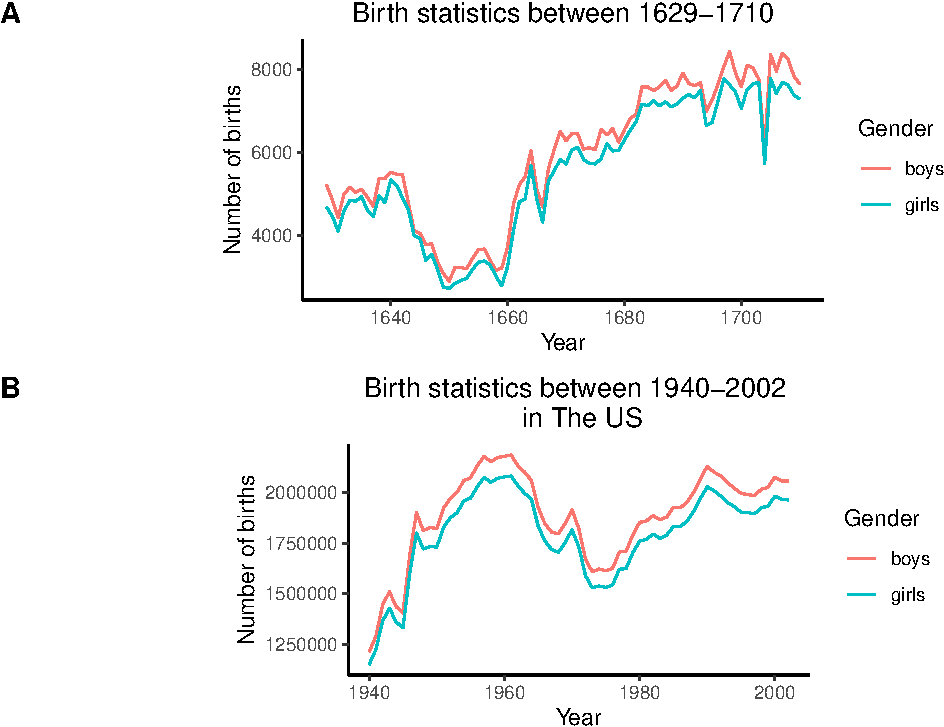
\includegraphics{Arindom_Baruah_32779267_files/figure-latex/figbirth-1} 

}

\caption{Total number of births in two time periods}\label{fig:figbirth}
\end{figure}

\normalsize

As we can observe through figure \ref{fig:figbirth}, the magnitude of births are observed to be \textbf{significantly higher during the period between 1940-2002 in the United States} when compared to the period between 1620-1710 of Arbuthnot's data.

\hypertarget{query-2}{%
\subsection{Query 2}\label{query-2}}

In this section, the number of births classified as ``girls'' will be focused on to gain further insights through a scatter plot as visualised through figure \ref{fig:girlbirth}.

\tiny

\begin{Shaded}
\begin{Highlighting}[]
\NormalTok{pl3 }\OtherTok{\textless{}{-}} \FunctionTok{ggplot}\NormalTok{(}\AttributeTok{data =}\NormalTok{ df\_present, }\FunctionTok{aes}\NormalTok{(}\AttributeTok{x =}\NormalTok{ year, }\AttributeTok{y =}\NormalTok{ girls)) }\SpecialCharTok{+}
  \FunctionTok{geom\_point}\NormalTok{(}\AttributeTok{shape =} \DecValTok{2}\NormalTok{, }\AttributeTok{color =} \StringTok{\textquotesingle{}red\textquotesingle{}}\NormalTok{) }\SpecialCharTok{+} \FunctionTok{theme\_classic}\NormalTok{() }\SpecialCharTok{+} 
  \FunctionTok{ggtitle}\NormalTok{(}\StringTok{"Number of girls born during 1940{-}2002 }\SpecialCharTok{\textbackslash{}n}\StringTok{ in the US"}\NormalTok{) }\SpecialCharTok{+} 
  \FunctionTok{theme}\NormalTok{(}\AttributeTok{plot.title =} \FunctionTok{element\_text}\NormalTok{(}\AttributeTok{hjust =} \FloatTok{0.5}\NormalTok{), }\AttributeTok{aspect.ratio =} \FloatTok{0.5}\NormalTok{) }\SpecialCharTok{+} \FunctionTok{labs}\NormalTok{(}\AttributeTok{x =} \StringTok{"Year"}\NormalTok{, }
                                                                           \AttributeTok{y =} \StringTok{"Number of births"}\NormalTok{)}
\NormalTok{pl4 }\OtherTok{\textless{}{-}} \FunctionTok{ggplot}\NormalTok{(}\AttributeTok{data =}\NormalTok{ df\_arb, }\FunctionTok{aes}\NormalTok{(}\AttributeTok{x =}\NormalTok{ year, }\AttributeTok{y =}\NormalTok{ girls)) }\SpecialCharTok{+}
  \FunctionTok{geom\_point}\NormalTok{(}\AttributeTok{shape =} \DecValTok{2}\NormalTok{, }\AttributeTok{color =} \StringTok{\textquotesingle{}blue\textquotesingle{}}\NormalTok{) }\SpecialCharTok{+} \FunctionTok{theme\_classic}\NormalTok{() }\SpecialCharTok{+} 
  \FunctionTok{ggtitle}\NormalTok{(}\StringTok{"Number of girls born during 1629{-}1710"}\NormalTok{) }\SpecialCharTok{+} 
  \FunctionTok{theme}\NormalTok{(}\AttributeTok{plot.title =} \FunctionTok{element\_text}\NormalTok{(}\AttributeTok{hjust =} \FloatTok{0.5}\NormalTok{), }\AttributeTok{aspect.ratio =} \FloatTok{0.5}\NormalTok{) }\SpecialCharTok{+} \FunctionTok{labs}\NormalTok{(}\AttributeTok{x =} \StringTok{"Year"}\NormalTok{, }
                                                                           \AttributeTok{y =} \StringTok{"Number of births"}\NormalTok{)}
\FunctionTok{plot\_grid}\NormalTok{(pl3,pl4,}\AttributeTok{ncol =}\DecValTok{1}\NormalTok{)}
\end{Highlighting}
\end{Shaded}

\begin{figure}

{\centering 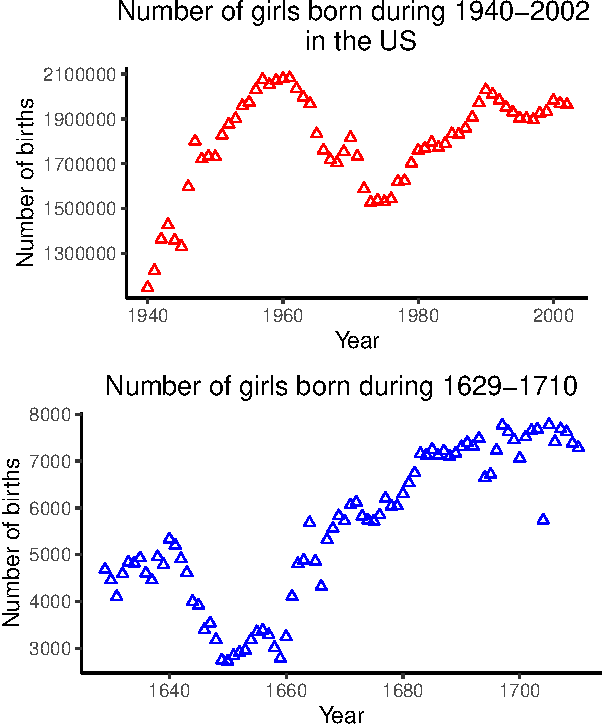
\includegraphics{Arindom_Baruah_32779267_files/figure-latex/girlbirth-1} 

}

\caption{Girls born during each periods}\label{fig:girlbirth}
\end{figure}
\normalsize

\newpage

\hypertarget{query-3}{%
\subsection{Query 3}\label{query-3}}

Based on the analysis of figures \ref{fig:girlbirth} and \ref{fig:pres}, we can observe the following key points:

\begin{enumerate}
\def\labelenumi{\arabic{enumi}.}
\tightlist
\item
  The magnitude of girls born in the period between 1940-2002 is \textbf{significantly higher} than in the period between 1629-1710.
\item
  Although the magnitude of girls born for the two time periods vary significantly, however a few similarities in the trends may be observed between the two time periods. These include the sudden dip in births followed by a rise and eventual stagnation of the numbers.
\item
  During the period between 1940-1960, there was \textbf{a consistent increase in the number of girls born in the country}.
\item
  The period between 1960-1975 observed a \textbf{sudden drop in the number of girls born}.
\item
  However, the number of girls born were \textbf{back on the rise} after the year 1975.
\item
  Between the period of 1990-2000, the \textbf{number of girls born were observed to stagnate at approximately 200,0000 births a year}.
\end{enumerate}

\tiny

\begin{Shaded}
\begin{Highlighting}[]
\NormalTok{pl5 }\OtherTok{\textless{}{-}} \FunctionTok{ggplot}\NormalTok{(}\AttributeTok{data =}\NormalTok{ df\_present, }\FunctionTok{aes}\NormalTok{(}\AttributeTok{x =}\NormalTok{ year, }\AttributeTok{y =}\NormalTok{ girls)) }\SpecialCharTok{+}
  \FunctionTok{geom\_point}\NormalTok{(}\AttributeTok{shape =} \DecValTok{2}\NormalTok{, }\AttributeTok{color =} \StringTok{\textquotesingle{}red\textquotesingle{}}\NormalTok{) }\SpecialCharTok{+} \FunctionTok{theme\_classic}\NormalTok{() }\SpecialCharTok{+} 
  \FunctionTok{ggtitle}\NormalTok{(}\StringTok{"Number of girls born during 1940{-}2002 }\SpecialCharTok{\textbackslash{}n}\StringTok{ in the US"}\NormalTok{) }\SpecialCharTok{+}
   \FunctionTok{labs}\NormalTok{(}\AttributeTok{x =} \StringTok{"Year"}\NormalTok{, }\AttributeTok{y =} \StringTok{"Number of births"}\NormalTok{) }\SpecialCharTok{+} \FunctionTok{theme}\NormalTok{(}\AttributeTok{plot.title =} \FunctionTok{element\_text}\NormalTok{(}\AttributeTok{hjust =} \FloatTok{0.5}\NormalTok{), }
                                                    \AttributeTok{aspect.ratio =} \FloatTok{0.7}\NormalTok{) }\SpecialCharTok{+}
  \FunctionTok{annotate}\NormalTok{(}
    \StringTok{"segment"}\NormalTok{,}
    \AttributeTok{x =} \DecValTok{1945}\NormalTok{,}
    \AttributeTok{y =} \DecValTok{1900000}\NormalTok{,}
    \AttributeTok{xend =} \DecValTok{1950}\NormalTok{  ,}
    \AttributeTok{yend =} \DecValTok{1800000}\NormalTok{,}
    \AttributeTok{arrow =} \FunctionTok{arrow}\NormalTok{(}\AttributeTok{type =} \StringTok{"closed"}\NormalTok{,}
                  \AttributeTok{length =} \FunctionTok{unit}\NormalTok{(}\FloatTok{0.02}\NormalTok{, }\StringTok{"npc"}\NormalTok{))}
\NormalTok{  ) }\SpecialCharTok{+}
  \FunctionTok{annotate}\NormalTok{(}
    \StringTok{"text"}\NormalTok{,}
    \AttributeTok{x =} \DecValTok{1946}\NormalTok{,}
    \AttributeTok{y =} \DecValTok{1980000}\NormalTok{,}
    \AttributeTok{colour =} \StringTok{"black"}\NormalTok{,}
    \AttributeTok{label =} \StringTok{\textquotesingle{}Consistent rise in number of girls }\SpecialCharTok{\textbackslash{}n}\StringTok{ born between 1940{-}1960\textquotesingle{}}\NormalTok{,}
    \AttributeTok{size =} \FunctionTok{unit}\NormalTok{(}\FloatTok{2.5}\NormalTok{, }\StringTok{"pt"}\NormalTok{)}
\NormalTok{  ) }\SpecialCharTok{+}
  \FunctionTok{annotate}\NormalTok{(}
    \StringTok{"segment"}\NormalTok{,}
    \AttributeTok{x =} \DecValTok{1965}\NormalTok{,}
    \AttributeTok{y =} \DecValTok{1300000}\NormalTok{,}
    \AttributeTok{xend =} \DecValTok{1973}\NormalTok{  ,}
    \AttributeTok{yend =} \DecValTok{1500000}\NormalTok{,}
    \AttributeTok{arrow =} \FunctionTok{arrow}\NormalTok{(}\AttributeTok{type =} \StringTok{"closed"}\NormalTok{,}
                  \AttributeTok{length =} \FunctionTok{unit}\NormalTok{(}\FloatTok{0.02}\NormalTok{, }\StringTok{"npc"}\NormalTok{))}
\NormalTok{  ) }\SpecialCharTok{+}
  \FunctionTok{annotate}\NormalTok{(}
    \StringTok{"text"}\NormalTok{,}
    \AttributeTok{x =} \DecValTok{1965}\NormalTok{,}
    \AttributeTok{y =} \DecValTok{1250000}\NormalTok{,}
    \AttributeTok{colour =} \StringTok{"blue"}\NormalTok{,}
    \AttributeTok{label =} \StringTok{\textquotesingle{}Dip in number of girls born }\SpecialCharTok{\textbackslash{}n}\StringTok{ between 1960{-}1975\textquotesingle{}}\NormalTok{,}
    \AttributeTok{size =} \FunctionTok{unit}\NormalTok{(}\FloatTok{2.5}\NormalTok{, }\StringTok{"pt"}\NormalTok{)}
\NormalTok{  ) }\SpecialCharTok{+}
  \FunctionTok{annotate}\NormalTok{(}
    \StringTok{"segment"}\NormalTok{,}
    \AttributeTok{x =} \DecValTok{1983}\NormalTok{,}
    \AttributeTok{y =} \DecValTok{1500000}\NormalTok{,}
    \AttributeTok{xend =} \DecValTok{1985}\NormalTok{  ,}
    \AttributeTok{yend =} \DecValTok{1700000}\NormalTok{,}
    \AttributeTok{arrow =} \FunctionTok{arrow}\NormalTok{(}\AttributeTok{type =} \StringTok{"closed"}\NormalTok{,}
                  \AttributeTok{length =} \FunctionTok{unit}\NormalTok{(}\FloatTok{0.02}\NormalTok{, }\StringTok{"npc"}\NormalTok{))}
\NormalTok{  ) }\SpecialCharTok{+}
  \FunctionTok{annotate}\NormalTok{(}
    \StringTok{"text"}\NormalTok{,}
    \AttributeTok{x =} \DecValTok{1985}\NormalTok{,}
    \AttributeTok{y =} \DecValTok{1450000}\NormalTok{,}
    \AttributeTok{colour =} \StringTok{"darkgreen"}\NormalTok{,}
    \AttributeTok{label =} \StringTok{\textquotesingle{}Girl child births start }\SpecialCharTok{\textbackslash{}n}\StringTok{ increasing again from 1975\textquotesingle{}}\NormalTok{,}
    \AttributeTok{size =} \FunctionTok{unit}\NormalTok{(}\FloatTok{2.5}\NormalTok{, }\StringTok{"pt"}\NormalTok{)}
\NormalTok{  ) }\SpecialCharTok{+}
    \FunctionTok{annotate}\NormalTok{(}
    \StringTok{"segment"}\NormalTok{,}
    \AttributeTok{x =} \DecValTok{1995}\NormalTok{,}
    \AttributeTok{y =} \DecValTok{1700000}\NormalTok{,}
    \AttributeTok{xend =} \DecValTok{1995}\NormalTok{  ,}
    \AttributeTok{yend =} \DecValTok{1850000}\NormalTok{,}
    \AttributeTok{arrow =} \FunctionTok{arrow}\NormalTok{(}\AttributeTok{type =} \StringTok{"closed"}\NormalTok{,}
                  \AttributeTok{length =} \FunctionTok{unit}\NormalTok{(}\FloatTok{0.02}\NormalTok{, }\StringTok{"npc"}\NormalTok{))}
\NormalTok{  ) }\SpecialCharTok{+}
  \FunctionTok{annotate}\NormalTok{(}
    \StringTok{"text"}\NormalTok{,}
    \AttributeTok{x =} \DecValTok{1995}\NormalTok{,}
    \AttributeTok{y =} \DecValTok{1600000}\NormalTok{,}
    \AttributeTok{colour =} \StringTok{"darkred"}\NormalTok{,}
    \AttributeTok{label =} \StringTok{\textquotesingle{}Stagnation in the number }\SpecialCharTok{\textbackslash{}n}\StringTok{ of girls born after 1990\textquotesingle{}}\NormalTok{,}
    \AttributeTok{size =} \FunctionTok{unit}\NormalTok{(}\FloatTok{2.5}\NormalTok{, }\StringTok{"pt"}\NormalTok{)}
\NormalTok{  )  }
\NormalTok{pl5}
\end{Highlighting}
\end{Shaded}

\begin{figure}

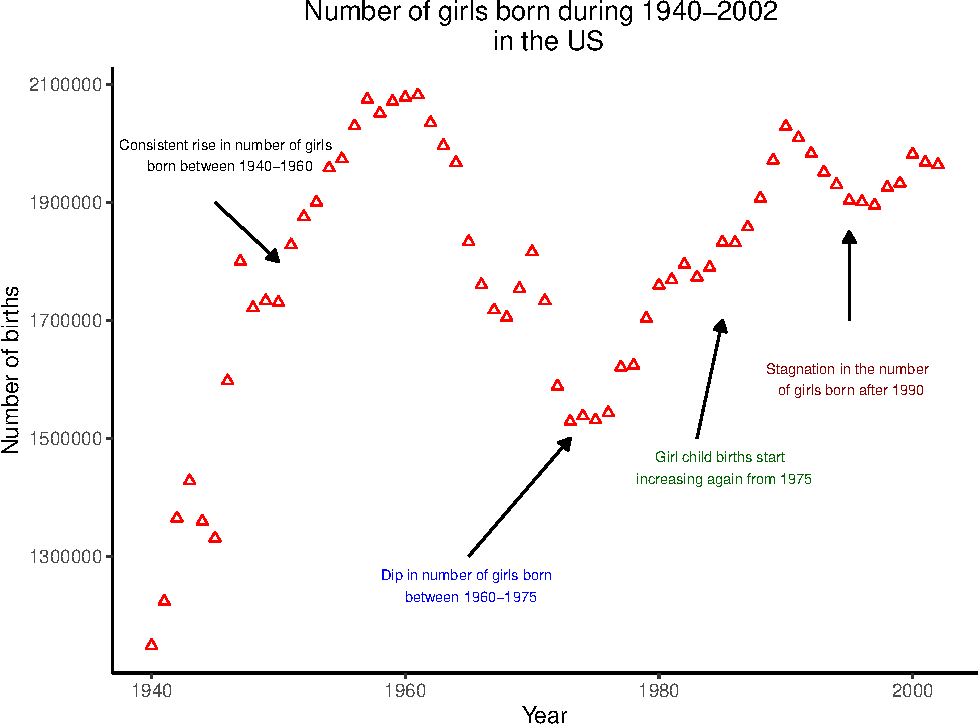
\includegraphics{Arindom_Baruah_32779267_files/figure-latex/pres-1} \hfill{}

\caption{Trend analysis of girls child births in The United States during 1940-2002}\label{fig:pres}
\end{figure}
\normalsize
\newpage

\hypertarget{query-4}{%
\subsection{Query 4}\label{query-4}}

While the raw dataset provides an overall understanding of the gender birth number in the United States, this section will focus on the creation of new statistical features which will help provide deeper insights. Based on the available data, a total of 4 new features will be created. These features may be described as follows:

\begin{enumerate}
\def\labelenumi{\arabic{enumi}.}
\tightlist
\item
  \textbf{Total} : Total number of child births for the corresponding year in the United States.
\item
  \textbf{Ratio} : This feature maybe defined as the ratio of the number of girls born to the number of boys born for a particular year.
\item
  \textbf{Prop\_girls}: This feature maybe defined as the ratio of the number of girls born to the total number of children born for a particular year.
\item
  \textbf{Prop\_boys}: This feature maybe defined as the ratio of the number of boys born to the total number of children born for a particular year.
\end{enumerate}

The above new features will be calculated through the following code chunk below and the data has been tabulated in table \ref{tab:feateng}.

\tiny

\begin{Shaded}
\begin{Highlighting}[]
\NormalTok{df\_present }\OtherTok{\textless{}{-}}\NormalTok{ df\_present }\SpecialCharTok{\%\textgreater{}\%} \FunctionTok{mutate}\NormalTok{(}\AttributeTok{Total =}\NormalTok{ boys }\SpecialCharTok{+}\NormalTok{ girls) }\SpecialCharTok{\%\textgreater{}\%} 
  \FunctionTok{mutate}\NormalTok{(}\AttributeTok{Ratio =}\NormalTok{ girls}\SpecialCharTok{/}\NormalTok{boys) }\SpecialCharTok{\%\textgreater{}\%} 
  \FunctionTok{mutate}\NormalTok{(}\AttributeTok{Prop\_girls =}\NormalTok{ girls}\SpecialCharTok{/}\NormalTok{Total) }\SpecialCharTok{\%\textgreater{}\%} 
  \FunctionTok{mutate}\NormalTok{(}\AttributeTok{Prop\_boys =}\NormalTok{ boys}\SpecialCharTok{/}\NormalTok{Total)}

\FunctionTok{head}\NormalTok{(df\_present) }\SpecialCharTok{\%\textgreater{}\%} \FunctionTok{kable}\NormalTok{(}\AttributeTok{caption =} \StringTok{"Addition of new features in the data for births between 1940{-}2002."}\NormalTok{) }\SpecialCharTok{\%\textgreater{}\%} 
  \FunctionTok{kable\_styling}\NormalTok{(}\AttributeTok{bootstrap\_options =} \FunctionTok{c}\NormalTok{(}\StringTok{"bordered"}\NormalTok{,}\StringTok{"hover"}\NormalTok{),}
                                    \AttributeTok{latex\_options =} \StringTok{"HOLD\_position"}\NormalTok{) }
\end{Highlighting}
\end{Shaded}

\begin{table}[H]

\caption{\label{tab:feateng}Addition of new features in the data for births between 1940-2002.}
\centering
\begin{tabular}[t]{r|r|r|r|r|r|r}
\hline
year & boys & girls & Total & Ratio & Prop\_girls & Prop\_boys\\
\hline
1940 & 1211684 & 1148715 & 2360399 & 0.9480318 & 0.4866614 & 0.5133386\\
\hline
1941 & 1289734 & 1223693 & 2513427 & 0.9487949 & 0.4868624 & 0.5131376\\
\hline
1942 & 1444365 & 1364631 & 2808996 & 0.9447965 & 0.4858074 & 0.5141926\\
\hline
1943 & 1508959 & 1427901 & 2936860 & 0.9462822 & 0.4861999 & 0.5138001\\
\hline
1944 & 1435301 & 1359499 & 2794800 & 0.9471874 & 0.4864387 & 0.5135613\\
\hline
1945 & 1404587 & 1330869 & 2735456 & 0.9475162 & 0.4865255 & 0.5134745\\
\hline
\end{tabular}
\end{table}
\normalsize

\hypertarget{query-5}{%
\subsection{Query 5}\label{query-5}}

This section shall aim to understand the difference between the number of boys and girls born during the period between 1940-2002 in The United States. For gaining in-depth insights, the proportionality of male births will be visualised. The code chunk below provides the visualisation technique to be used for understanding the change in child sex-ratio during the period of interest.

\tiny

\begin{Shaded}
\begin{Highlighting}[]
\NormalTok{pl6 }\OtherTok{\textless{}{-}} \FunctionTok{ggplot}\NormalTok{(}\AttributeTok{data =}\NormalTok{ df\_present,}\FunctionTok{aes}\NormalTok{(}\AttributeTok{x =}\NormalTok{ year, }\AttributeTok{y =}\NormalTok{ Prop\_boys)) }\SpecialCharTok{+} 
  \FunctionTok{geom\_line}\NormalTok{(}\AttributeTok{size=}\FloatTok{1.5}\NormalTok{,}\AttributeTok{alpha=}\FloatTok{0.6}\NormalTok{) }\SpecialCharTok{+} \FunctionTok{ylim}\NormalTok{(}\FloatTok{0.475}\NormalTok{,}\FloatTok{0.53}\NormalTok{) }\SpecialCharTok{+} \FunctionTok{theme\_classic}\NormalTok{() }\SpecialCharTok{+} \FunctionTok{geom\_point}\NormalTok{(}\AttributeTok{color =} \StringTok{"darkred"}\NormalTok{,}\AttributeTok{size=}\DecValTok{1}\NormalTok{) }\SpecialCharTok{+}
  \FunctionTok{geom\_hline}\NormalTok{(}\AttributeTok{yintercept =} \FloatTok{0.5}\NormalTok{,}
             \AttributeTok{color =} \StringTok{\textquotesingle{}blue\textquotesingle{}}\NormalTok{,}
             \AttributeTok{linetype =} \StringTok{"twodash"}\NormalTok{,}
             \AttributeTok{size =} \DecValTok{2}\NormalTok{,}\AttributeTok{alpha=}\FloatTok{0.6}\NormalTok{) }\SpecialCharTok{+} \FunctionTok{labs}\NormalTok{(}\AttributeTok{x =} \StringTok{"Year"}\NormalTok{, }\AttributeTok{y=} \StringTok{"Proportion of boys"}\NormalTok{) }\SpecialCharTok{+} 
  \FunctionTok{ggtitle}\NormalTok{(}\StringTok{"Proportion of boys in the US }\SpecialCharTok{\textbackslash{}n}\StringTok{ between 1940{-}2002"}\NormalTok{) }\SpecialCharTok{+} 
  \FunctionTok{theme}\NormalTok{(}\AttributeTok{plot.title =} \FunctionTok{element\_text}\NormalTok{(}\AttributeTok{hjust =} \FloatTok{0.5}\NormalTok{)) }\SpecialCharTok{+}
  
  \FunctionTok{annotate}\NormalTok{(}
    \StringTok{"text"}\NormalTok{,}
    \AttributeTok{x =} \DecValTok{1980}\NormalTok{,}
    \AttributeTok{y =} \FloatTok{0.52}\NormalTok{,}
    \AttributeTok{colour =} \StringTok{"darkred"}\NormalTok{,}
    \AttributeTok{label =} \StringTok{\textquotesingle{}Higher proportion of boys born }\SpecialCharTok{\textbackslash{}n}\StringTok{ between 1940{-}2002\textquotesingle{}}\NormalTok{,}
    \AttributeTok{size =} \FunctionTok{unit}\NormalTok{(}\FloatTok{2.5}\NormalTok{, }\StringTok{"pt"}\NormalTok{)}
\NormalTok{  ) }\SpecialCharTok{+} \FunctionTok{theme}\NormalTok{(}\AttributeTok{aspect.ratio =} \DecValTok{1}\NormalTok{)}
\NormalTok{pl6}
\end{Highlighting}
\end{Shaded}

\begin{figure}

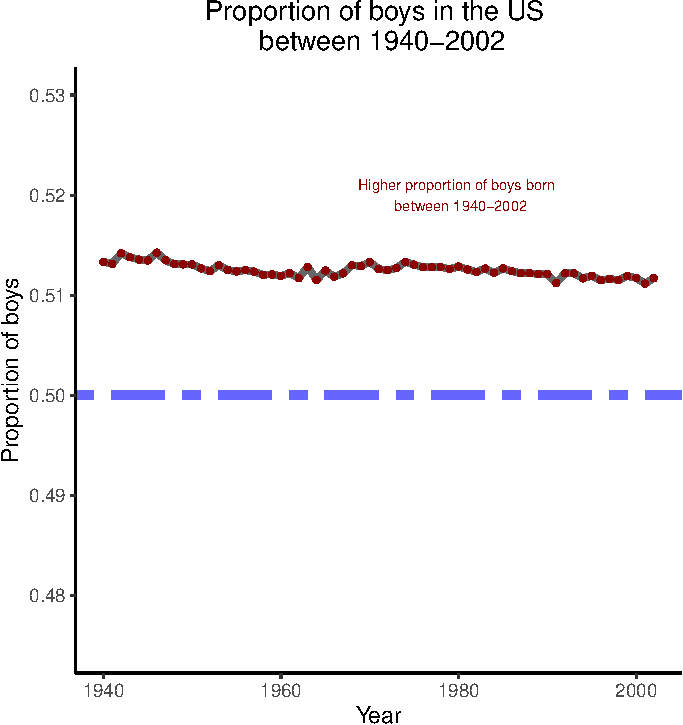
\includegraphics{Arindom_Baruah_32779267_files/figure-latex/propboys-1} \hfill{}

\caption{Proportion of boys born between 1940-2002}\label{fig:propboys}
\end{figure}
\normalsize

Figure \ref{fig:propboys} suggests that the proportion of boys and consequently, the number of boys born in the United States during the period between 1940-2002 is \textbf{indeed greater than the proportion of girls born in the same time period}. As a result, the observations pertaining to the birth statistics of the United States between the period of 1940-2002 \textbf{closely corroborates} with the findings of \textcite{arbuthnot1710ii} during the period of 1629-1710.

\hypertarget{conclusion}{%
\section{Conclusion}\label{conclusion}}

The key takeaways from the above analysis are as follows:

\begin{enumerate}
\def\labelenumi{\arabic{enumi}.}
\tightlist
\item
  The magnitude of children born are significantly greater in the period of 1940-2002 when compared to the period of 1629-1710.
\item
  Statistics pertaining to female child birth were observed to undergo a sudden dip and then subsequently rise and stagnate for both the time periods. Hence, the two time periods were observed to report similarities in its trend.
\item
  Proportion of male child birth continue to be greater than female child birth in The United States during the period of 1940-2002. A similar observation was first reported by \textcite{arbuthnot1710ii} for the period of 1629-1710.
\end{enumerate}

\hypertarget{resources}{%
\section{Resources}\label{resources}}

The above analysis was undertaken with the help of the following software and packages:

\begin{enumerate}
\def\labelenumi{\arabic{enumi}.}
\tightlist
\item
  \textbf{RStudio}: Integrated Development for R. RStudio, PBC, Boston, MA URL \url{http://www.rstudio.com/}.
\item
  \textbf{ggplot2}: H. Wickham. ggplot2: Elegant Graphics for Data Analysis. Springer-Verlag New York, 2016.
\item
  \textbf{tidyverse}: Wickham H, Averick M, Bryan J, Chang W, McGowan LD, François R, Grolemund G, Hayes A, Henry L, Hester J, Kuhn M, Pedersen TL, Miller E, Bache SM, Müller K,
  Ooms J, Robinson D, Seidel DP, Spinu V, Takahashi K, Vaughan D, Wilke C, Woo K, Yutani H (2019). ``Welcome to the tidyverse.'' \emph{Journal of Open Source Software},
  \emph{4}(43), 1686. \url{doi:10.21105/joss.01686} \url{https://doi.org/10.21105/joss.01686}.
\item
  \textbf{here}: Müller K (2020). \emph{here: A Simpler Way to Find Your Files}. R package version 1.0.1, \url{https://CRAN.R-project.org/package=here}.
\item
  \textbf{knitr}: Yihui Xie (2014) knitr: A Comprehensive Tool for Reproducible Research in R. In Victoria Stodden, Friedrich Leisch and Roger D. Peng, editors, Implementing
  Reproducible Computational Research. Chapman and Hall/CRC. ISBN 978-1466561595.
\item
  \textbf{rmarkdown}: Allaire J, Xie Y, Dervieux C, McPherson J, Luraschi J, Ushey K, Atkins A, Wickham H, Cheng J, Chang W, Iannone R (2023). \emph{rmarkdown: Dynamic Documents for R}.
  R package version 2.23, \url{https://github.com/rstudio/rmarkdown}.
\item
  \textbf{cowplot}: Wilke C (2020). \emph{cowplot: Streamlined Plot Theme and Plot Annotations for `ggplot2'}. R package version 1.1.1, \url{https://CRAN.R-project.org/package=cowplot}.
\item
  \textbf{kableExtra}: Zhu H (2023). \emph{kableExtra: Construct Complex Table with `kable' and Pipe Syntax}. \url{http://haozhu233.github.io/kableExtra}
\end{enumerate}

\printbibliography

\end{document}
